\documentclass[1p]{elsarticle_modified}
%\bibliographystyle{elsarticle-num}

%\usepackage[colorlinks]{hyperref}
%\usepackage{abbrmath_seonhwa} %\Abb, \Ascr, \Acal ,\Abf, \Afrak
\usepackage{amsfonts}
\usepackage{amssymb}
\usepackage{amsmath}
\usepackage{amsthm}
\usepackage{scalefnt}
\usepackage{amsbsy}
\usepackage{kotex}
\usepackage{caption}
\usepackage{subfig}
\usepackage{color}
\usepackage{graphicx}
\usepackage{xcolor} %% white, black, red, green, blue, cyan, magenta, yellow
\usepackage{float}
\usepackage{setspace}
\usepackage{hyperref}

\usepackage{tikz}
\usetikzlibrary{arrows}

\usepackage{multirow}
\usepackage{array} % fixed length table
\usepackage{hhline}

%%%%%%%%%%%%%%%%%%%%%
\makeatletter
\renewcommand*\env@matrix[1][\arraystretch]{%
	\edef\arraystretch{#1}%
	\hskip -\arraycolsep
	\let\@ifnextchar\new@ifnextchar
	\array{*\c@MaxMatrixCols c}}
\makeatother %https://tex.stackexchange.com/questions/14071/how-can-i-increase-the-line-spacing-in-a-matrix
%%%%%%%%%%%%%%%

\usepackage[normalem]{ulem}

\newcommand{\msout}[1]{\ifmmode\text{\sout{\ensuremath{#1}}}\else\sout{#1}\fi}
%SOURCE: \msout is \stkout macro in https://tex.stackexchange.com/questions/20609/strikeout-in-math-mode

\newcommand{\cancel}[1]{
	\ifmmode
	{\color{red}\msout{#1}}
	\else
	{\color{red}\sout{#1}}
	\fi
}

\newcommand{\add}[1]{
	{\color{blue}\uwave{#1}}
}

\newcommand{\replace}[2]{
	\ifmmode
	{\color{red}\msout{#1}}{\color{blue}\uwave{#2}}
	\else
	{\color{red}\sout{#1}}{\color{blue}\uwave{#2}}
	\fi
}

\newcommand{\Sol}{\mathcal{S}} %segment
\newcommand{\D}{D} %diagram
\newcommand{\A}{\mathcal{A}} %arc


%%%%%%%%%%%%%%%%%%%%%%%%%%%%%5 test

\def\sl{\operatorname{\textup{SL}}(2,\Cbb)}
\def\psl{\operatorname{\textup{PSL}}(2,\Cbb)}
\def\quan{\mkern 1mu \triangleright \mkern 1mu}

\theoremstyle{definition}
\newtheorem{thm}{Theorem}[section]
\newtheorem{prop}[thm]{Proposition}
\newtheorem{lem}[thm]{Lemma}
\newtheorem{ques}[thm]{Question}
\newtheorem{cor}[thm]{Corollary}
\newtheorem{defn}[thm]{Definition}
\newtheorem{exam}[thm]{Example}
\newtheorem{rmk}[thm]{Remark}
\newtheorem{alg}[thm]{Algorithm}

\newcommand{\I}{\sqrt{-1}}
\begin{document}

%\begin{frontmatter}
%
%\title{Boundary parabolic representations of knots up to 8 crossings}
%
%%% Group authors per affiliation:
%\author{Yunhi Cho} 
%\address{Department of Mathematics, University of Seoul, Seoul, Korea}
%\ead{yhcho@uos.ac.kr}
%
%
%\author{Seonhwa Kim} %\fnref{s_kim}}
%\address{Center for Geometry and Physics, Institute for Basic Science, Pohang, 37673, Korea}
%\ead{ryeona17@ibs.re.kr}
%
%\author{Hyuk Kim}
%\address{Department of Mathematical Sciences, Seoul National University, Seoul 08826, Korea}
%\ead{hyukkim@snu.ac.kr}
%
%\author{Seokbeom Yoon}
%\address{Department of Mathematical Sciences, Seoul National University, Seoul, 08826,  Korea}
%\ead{sbyoon15@snu.ac.kr}
%
%\begin{abstract}
%We find all boundary parabolic representation of knots up to 8 crossings.
%
%\end{abstract}
%\begin{keyword}
%    \MSC[2010] 57M25 
%\end{keyword}
%
%\end{frontmatter}

%\linenumbers
%\tableofcontents
%
\newcommand\colored[1]{\textcolor{white}{\rule[-0.35ex]{0.8em}{1.4ex}}\kern-0.8em\color{red} #1}%
%\newcommand\colored[1]{\textcolor{white}{ #1}\kern-2.17ex	\textcolor{white}{ #1}\kern-1.81ex	\textcolor{white}{ #1}\kern-2.15ex\color{red}#1	}

{\Large $\underline{11n_{119}~(K11n_{119})}$}

\setlength{\tabcolsep}{10pt}
\renewcommand{\arraystretch}{1.6}
\vspace{1cm}\begin{tabular}{m{100pt}>{\centering\arraybackslash}m{274pt}}
\multirow{5}{120pt}{
	\centering
	\includegraphics[width=112pt]{../../../GIT/diagram.site/Diagrams/png/735_11n_119.png}\\
\ \ \ A knot diagram\footnotemark}&
\allowdisplaybreaks
\textbf{Linearized knot diagam} \\
\cline{2-2}
 &
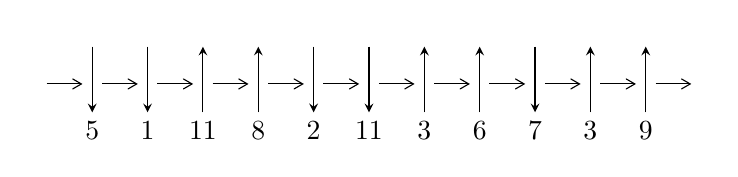
\begin{tikzpicture}[x=20pt, y=17pt]
	% nodes
	\node (C0) at (0, 0) {};
	\node (C1) at (1, 0) {};
	\node (C1U) at (1, +1) {};
	\node (C1D) at (1, -1) {5};

	\node (C2) at (2, 0) {};
	\node (C2U) at (2, +1) {};
	\node (C2D) at (2, -1) {1};

	\node (C3) at (3, 0) {};
	\node (C3U) at (3, +1) {};
	\node (C3D) at (3, -1) {11};

	\node (C4) at (4, 0) {};
	\node (C4U) at (4, +1) {};
	\node (C4D) at (4, -1) {8};

	\node (C5) at (5, 0) {};
	\node (C5U) at (5, +1) {};
	\node (C5D) at (5, -1) {2};

	\node (C6) at (6, 0) {};
	\node (C6U) at (6, +1) {};
	\node (C6D) at (6, -1) {11};

	\node (C7) at (7, 0) {};
	\node (C7U) at (7, +1) {};
	\node (C7D) at (7, -1) {3};

	\node (C8) at (8, 0) {};
	\node (C8U) at (8, +1) {};
	\node (C8D) at (8, -1) {6};

	\node (C9) at (9, 0) {};
	\node (C9U) at (9, +1) {};
	\node (C9D) at (9, -1) {7};

	\node (C10) at (10, 0) {};
	\node (C10U) at (10, +1) {};
	\node (C10D) at (10, -1) {3};

	\node (C11) at (11, 0) {};
	\node (C11U) at (11, +1) {};
	\node (C11D) at (11, -1) {9};
	\node (C12) at (12, 0) {};

	% arrows
	\draw[->,>={angle 60}]
	(C0) edge (C1) (C1) edge (C2) (C2) edge (C3) (C3) edge (C4) (C4) edge (C5) (C5) edge (C6) (C6) edge (C7) (C7) edge (C8) (C8) edge (C9) (C9) edge (C10) (C10) edge (C11) (C11) edge (C12) ;	\draw[->,>=stealth]
	(C1U) edge (C1D) (C2U) edge (C2D) (C3D) edge (C3U) (C4D) edge (C4U) (C5U) edge (C5D) (C6U) edge (C6D) (C7D) edge (C7U) (C8D) edge (C8U) (C9U) edge (C9D) (C10D) edge (C10U) (C11D) edge (C11U) ;
	\end{tikzpicture} \\
\hhline{~~} \\& 
\textbf{Solving Sequence} \\ \cline{2-2} 
 &
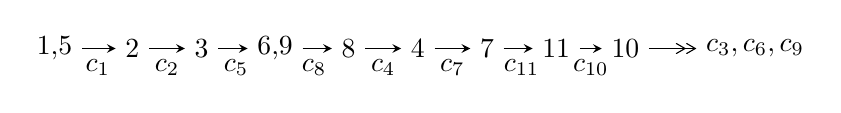
\begin{tikzpicture}[x=25pt, y=7pt]
	% node
	\node (A0) at (-1/8, 0) {1,5};
	\node (A1) at (1, 0) {2};
	\node (A2) at (2, 0) {3};
	\node (A3) at (49/16, 0) {6,9};
	\node (A4) at (33/8, 0) {8};
	\node (A5) at (41/8, 0) {4};
	\node (A6) at (49/8, 0) {7};
	\node (A7) at (57/8, 0) {11};
	\node (A8) at (65/8, 0) {10};
	\node (C1) at (1/2, -1) {$c_{1}$};
	\node (C2) at (3/2, -1) {$c_{2}$};
	\node (C3) at (5/2, -1) {$c_{5}$};
	\node (C4) at (29/8, -1) {$c_{8}$};
	\node (C5) at (37/8, -1) {$c_{4}$};
	\node (C6) at (45/8, -1) {$c_{7}$};
	\node (C7) at (53/8, -1) {$c_{11}$};
	\node (C8) at (61/8, -1) {$c_{10}$};
	\node (A9) at (10, 0) {$c_{3},c_{6},c_{9}$};

	% edge
	\draw[->,>=stealth]	
	(A0) edge (A1) (A1) edge (A2) (A2) edge (A3) (A3) edge (A4) (A4) edge (A5) (A5) edge (A6) (A6) edge (A7) (A7) edge (A8) ;
	\draw[->>,>={angle 60}]	
	(A8) edge (A9);
\end{tikzpicture} \\ 

\end{tabular} \\

\footnotetext{
The image of knot diagram is generated by the software ``\textbf{Draw programme}" developed by Andrew Bartholomew(\url{http://www.layer8.co.uk/maths/draw/index.htm\#Running-draw}), where we modified some parts for our purpose(\url{https://github.com/CATsTAILs/LinksPainter}).
}\phantom \\ \newline 
\centering \textbf{Ideals for irreducible components\footnotemark of $X_{\text{par}}$} 
 
\begin{align*}
I^u_{1}&=\langle 
2 u^{21}-8 u^{20}+\cdots+b+1,\;-25 u^{21}+124 u^{20}+\cdots+2 a+34,\;u^{22}-6 u^{21}+\cdots-10 u+2\rangle \\
I^u_{2}&=\langle 
u^9-3 u^7- u^6+5 u^5+3 u^4-5 u^3-5 u^2+b+u+3,\\
\phantom{I^u_{2}}&\phantom{= \langle  }- u^9-3 u^8+4 u^7+5 u^6-5 u^5-12 u^4+4 u^3+8 u^2+2 a+3 u-6,\\
\phantom{I^u_{2}}&\phantom{= \langle  }u^{10}+u^9-2 u^8-3 u^7+3 u^6+6 u^5-6 u^3-3 u^2+2 u+2\rangle \\
I^u_{3}&=\langle 
u^{10}+u^9- u^8-2 u^7+u^5+u^4- u^2 a- a u- u^2+b- u-1,\;u^{10} a- u^{10}+\cdots+a+1,\\
\phantom{I^u_{3}}&\phantom{= \langle  }u^{11}+u^{10}-2 u^9-3 u^8+2 u^7+4 u^6-3 u^4- u^3+u^2-1\rangle \\
\\
\end{align*}
\raggedright * 3 irreducible components of $\dim_{\mathbb{C}}=0$, with total 54 representations.\\
\footnotetext{All coefficients of polynomials are rational numbers. But the coefficients are sometimes approximated in decimal forms when there is not enough margin.}
\newpage
\renewcommand{\arraystretch}{1}
\centering \section*{I. $I^u_{1}= \langle 2 u^{21}-8 u^{20}+\cdots+b+1,\;-25 u^{21}+124 u^{20}+\cdots+2 a+34,\;u^{22}-6 u^{21}+\cdots-10 u+2 \rangle$}
\flushleft \textbf{(i) Arc colorings}\\
\begin{tabular}{m{7pt} m{180pt} m{7pt} m{180pt} }
\flushright $a_{1}=$&$\begin{pmatrix}1\\0\end{pmatrix}$ \\
\flushright $a_{5}=$&$\begin{pmatrix}0\\u\end{pmatrix}$ \\
\flushright $a_{2}=$&$\begin{pmatrix}1\\u^2\end{pmatrix}$ \\
\flushright $a_{3}=$&$\begin{pmatrix}- u^2+1\\u^2\end{pmatrix}$ \\
\flushright $a_{6}=$&$\begin{pmatrix}- u\\- u^3+u\end{pmatrix}$ \\
\flushright $a_{9}=$&$\begin{pmatrix}\frac{25}{2} u^{21}-62 u^{20}+\cdots+82 u-17\\-2 u^{21}+8 u^{20}+\cdots-3 u-1\end{pmatrix}$ \\
\flushright $a_{8}=$&$\begin{pmatrix}\frac{17}{2} u^{21}-44 u^{20}+\cdots+61 u-13\\-6 u^{21}+29 u^{20}+\cdots-34 u+7\end{pmatrix}$ \\
\flushright $a_{4}=$&$\begin{pmatrix}-\frac{1}{2} u^{21}+5 u^{20}+\cdots-18 u+5\\u^{21}-6 u^{20}+\cdots+13 u-3\end{pmatrix}$ \\
\flushright $a_{7}=$&$\begin{pmatrix}\frac{21}{2} u^{21}-54 u^{20}+\cdots+76 u-16\\-5 u^{21}+23 u^{20}+\cdots-20 u+3\end{pmatrix}$ \\
\flushright $a_{11}=$&$\begin{pmatrix}-\frac{5}{2} u^{21}+12 u^{20}+\cdots-18 u+5\\- u^{21}+5 u^{20}+\cdots-4 u+1\end{pmatrix}$ \\
\flushright $a_{10}=$&$\begin{pmatrix}-\frac{9}{2} u^{21}+22 u^{20}+\cdots-33 u+8\\-2 u^{21}+11 u^{20}+\cdots-18 u+5\end{pmatrix}$\\ \flushright $a_{10}=$&$\begin{pmatrix}-\frac{9}{2} u^{21}+22 u^{20}+\cdots-33 u+8\\-2 u^{21}+11 u^{20}+\cdots-18 u+5\end{pmatrix}$\\&\end{tabular}
\flushleft \textbf{(ii) Obstruction class $= -1$}\\~\\
\flushleft \textbf{(iii) Cusp Shapes $= 14 u^{21}-71 u^{20}+112 u^{19}+92 u^{18}-557 u^{17}+596 u^{16}+457 u^{15}-1669 u^{14}+1075 u^{13}+1272 u^{12}-2511 u^{11}+829 u^{10}+1721 u^9-2088 u^8+347 u^7+1061 u^6-920 u^5+128 u^4+294 u^3-268 u^2+118 u-26$}\\~\\
\newpage\renewcommand{\arraystretch}{1}
\flushleft \textbf{(iv) u-Polynomials at the component}\newline \\
\begin{tabular}{m{50pt}|m{274pt}}
Crossings & \hspace{64pt}u-Polynomials at each crossing \\
\hline $$\begin{aligned}c_{1},c_{5}\end{aligned}$$&$\begin{aligned}
&u^{22}+6 u^{21}+\cdots+10 u+2
\end{aligned}$\\
\hline $$\begin{aligned}c_{2}\end{aligned}$$&$\begin{aligned}
&u^{22}+10 u^{21}+\cdots-12 u+4
\end{aligned}$\\
\hline $$\begin{aligned}c_{3},c_{7},c_{10}\end{aligned}$$&$\begin{aligned}
&u^{22}+u^{21}+\cdots-2 u+1
\end{aligned}$\\
\hline $$\begin{aligned}c_{4}\end{aligned}$$&$\begin{aligned}
&u^{22}- u^{21}+\cdots-2 u+7
\end{aligned}$\\
\hline $$\begin{aligned}c_{6}\end{aligned}$$&$\begin{aligned}
&u^{22}+24 u^{21}+\cdots+22528 u+2048
\end{aligned}$\\
\hline $$\begin{aligned}c_{8},c_{11}\end{aligned}$$&$\begin{aligned}
&u^{22}+2 u^{21}+\cdots+2 u+1
\end{aligned}$\\
\hline $$\begin{aligned}c_{9}\end{aligned}$$&$\begin{aligned}
&u^{22}-11 u^{21}+\cdots+122 u+26
\end{aligned}$\\
\hline
\end{tabular}\\~\\
\newpage\renewcommand{\arraystretch}{1}
\flushleft \textbf{(v) Riley Polynomials at the component}\newline \\
\begin{tabular}{m{50pt}|m{274pt}}
Crossings & \hspace{64pt}Riley Polynomials at each crossing \\
\hline $$\begin{aligned}c_{1},c_{5}\end{aligned}$$&$\begin{aligned}
&y^{22}-10 y^{21}+\cdots+12 y+4
\end{aligned}$\\
\hline $$\begin{aligned}c_{2}\end{aligned}$$&$\begin{aligned}
&y^{22}+10 y^{21}+\cdots-304 y+16
\end{aligned}$\\
\hline $$\begin{aligned}c_{3},c_{7},c_{10}\end{aligned}$$&$\begin{aligned}
&y^{22}+35 y^{21}+\cdots+4 y+1
\end{aligned}$\\
\hline $$\begin{aligned}c_{4}\end{aligned}$$&$\begin{aligned}
&y^{22}+11 y^{21}+\cdots+276 y+49
\end{aligned}$\\
\hline $$\begin{aligned}c_{6}\end{aligned}$$&$\begin{aligned}
&y^{22}-4 y^{21}+\cdots+6291456 y+4194304
\end{aligned}$\\
\hline $$\begin{aligned}c_{8},c_{11}\end{aligned}$$&$\begin{aligned}
&y^{22}+6 y^{21}+\cdots+10 y+1
\end{aligned}$\\
\hline $$\begin{aligned}c_{9}\end{aligned}$$&$\begin{aligned}
&y^{22}-19 y^{21}+\cdots-13636 y+676
\end{aligned}$\\
\hline
\end{tabular}\\~\\
\newpage\flushleft \textbf{(vi) Complex Volumes and Cusp Shapes}
$$\begin{array}{c|c|c}  
\text{Solutions to }I^u_{1}& \I (\text{vol} + \sqrt{-1}CS) & \text{Cusp shape}\\
 \hline 
\begin{aligned}
u &= \phantom{-}0.415944 + 0.915063 I \\
a &= -1.072660 - 0.878457 I \\
b &= \phantom{-}1.02363 + 1.11399 I\end{aligned}
 & -5.47166 + 8.64336 I & \phantom{-}0.86416 - 4.17929 I \\ \hline\begin{aligned}
u &= \phantom{-}0.415944 - 0.915063 I \\
a &= -1.072660 + 0.878457 I \\
b &= \phantom{-}1.02363 - 1.11399 I\end{aligned}
 & -5.47166 - 8.64336 I & \phantom{-}0.86416 + 4.17929 I \\ \hline\begin{aligned}
u &= -0.905217 + 0.345552 I \\
a &= -0.583392 + 0.385060 I \\
b &= -0.562525 + 1.184670 I\end{aligned}
 & -1.27214 - 0.90119 I & \phantom{-}0.90722 - 4.11146 I \\ \hline\begin{aligned}
u &= -0.905217 - 0.345552 I \\
a &= -0.583392 - 0.385060 I \\
b &= -0.562525 - 1.184670 I\end{aligned}
 & -1.27214 + 0.90119 I & \phantom{-}0.90722 + 4.11146 I \\ \hline\begin{aligned}
u &= \phantom{-}0.938475 + 0.452741 I \\
a &= -1.211750 - 0.402886 I \\
b &= \phantom{-}0.478302 - 0.375259 I\end{aligned}
 & -1.47927 - 1.70785 I & -2.03135 + 1.38197 I \\ \hline\begin{aligned}
u &= \phantom{-}0.938475 - 0.452741 I \\
a &= -1.211750 + 0.402886 I \\
b &= \phantom{-}0.478302 + 0.375259 I\end{aligned}
 & -1.47927 + 1.70785 I & -2.03135 - 1.38197 I \\ \hline\begin{aligned}
u &= -0.961052 + 0.415714 I \\
a &= \phantom{-}0.289661 - 0.427398 I \\
b &= -0.023327 - 1.083510 I\end{aligned}
 & -1.68977 + 3.84529 I & \phantom{-}0.76962 - 7.11396 I \\ \hline\begin{aligned}
u &= -0.961052 - 0.415714 I \\
a &= \phantom{-}0.289661 + 0.427398 I \\
b &= -0.023327 + 1.083510 I\end{aligned}
 & -1.68977 - 3.84529 I & \phantom{-}0.76962 + 7.11396 I \\ \hline\begin{aligned}
u &= \phantom{-}1.006010 + 0.554191 I \\
a &= \phantom{-}2.06591 + 0.80886 I \\
b &= -1.075660 + 0.915138 I\end{aligned}
 & \phantom{-}0.29997 - 6.36774 I & -0.69331 + 5.66304 I \\ \hline\begin{aligned}
u &= \phantom{-}1.006010 - 0.554191 I \\
a &= \phantom{-}2.06591 - 0.80886 I \\
b &= -1.075660 - 0.915138 I\end{aligned}
 & \phantom{-}0.29997 + 6.36774 I & -0.69331 - 5.66304 I\\
 \hline 
 \end{array}$$\newpage$$\begin{array}{c|c|c}  
\text{Solutions to }I^u_{1}& \I (\text{vol} + \sqrt{-1}CS) & \text{Cusp shape}\\
 \hline 
\begin{aligned}
u &= \phantom{-}0.574081 + 0.572331 I \\
a &= \phantom{-}1.42670 + 1.36654 I \\
b &= -0.932058 - 0.660781 I\end{aligned}
 & \phantom{-}1.59219 + 1.82500 I & \phantom{-}1.63588 - 1.17331 I \\ \hline\begin{aligned}
u &= \phantom{-}0.574081 - 0.572331 I \\
a &= \phantom{-}1.42670 - 1.36654 I \\
b &= -0.932058 + 0.660781 I\end{aligned}
 & \phantom{-}1.59219 - 1.82500 I & \phantom{-}1.63588 + 1.17331 I \\ \hline\begin{aligned}
u &= \phantom{-}0.699271 + 0.989399 I \\
a &= -0.599352 + 0.221705 I \\
b &= \phantom{-}0.625328 - 0.499987 I\end{aligned}
 & -3.87629 - 3.75640 I & \phantom{-}1.54792 + 9.99919 I \\ \hline\begin{aligned}
u &= \phantom{-}0.699271 - 0.989399 I \\
a &= -0.599352 - 0.221705 I \\
b &= \phantom{-}0.625328 + 0.499987 I\end{aligned}
 & -3.87629 + 3.75640 I & \phantom{-}1.54792 - 9.99919 I \\ \hline\begin{aligned}
u &= -1.286580 + 0.073564 I \\
a &= \phantom{-}0.264997 - 0.359215 I \\
b &= \phantom{-}0.683728 - 1.124470 I\end{aligned}
 & -11.60060 - 5.70915 I & -5.06976 + 3.70908 I \\ \hline\begin{aligned}
u &= -1.286580 - 0.073564 I \\
a &= \phantom{-}0.264997 + 0.359215 I \\
b &= \phantom{-}0.683728 + 1.124470 I\end{aligned}
 & -11.60060 + 5.70915 I & -5.06976 - 3.70908 I \\ \hline\begin{aligned}
u &= \phantom{-}1.149220 + 0.647666 I \\
a &= -1.73202 - 0.77137 I \\
b &= \phantom{-}1.07821 - 1.26524 I\end{aligned}
 & -7.7036 - 14.3682 I & -1.51520 + 7.73205 I \\ \hline\begin{aligned}
u &= \phantom{-}1.149220 - 0.647666 I \\
a &= -1.73202 + 0.77137 I \\
b &= \phantom{-}1.07821 + 1.26524 I\end{aligned}
 & -7.7036 + 14.3682 I & -1.51520 - 7.73205 I \\ \hline\begin{aligned}
u &= \phantom{-}1.26179 + 0.79306 I \\
a &= \phantom{-}0.366388 - 0.137263 I \\
b &= \phantom{-}0.056443 + 0.483696 I\end{aligned}
 & -5.45392 - 3.28389 I & -19.7402 + 5.4613 I \\ \hline\begin{aligned}
u &= \phantom{-}1.26179 - 0.79306 I \\
a &= \phantom{-}0.366388 + 0.137263 I \\
b &= \phantom{-}0.056443 - 0.483696 I\end{aligned}
 & -5.45392 + 3.28389 I & -19.7402 - 5.4613 I\\
 \hline 
 \end{array}$$\newpage$$\begin{array}{c|c|c}  
\text{Solutions to }I^u_{1}& \I (\text{vol} + \sqrt{-1}CS) & \text{Cusp shape}\\
 \hline 
\begin{aligned}
u &= \phantom{-}0.108057 + 0.452974 I \\
a &= -0.214492 - 1.173680 I \\
b &= -0.352068 + 0.430105 I\end{aligned}
 & \phantom{-}0.466609 - 1.223850 I & \phantom{-}4.32498 + 5.87640 I \\ \hline\begin{aligned}
u &= \phantom{-}0.108057 - 0.452974 I \\
a &= -0.214492 + 1.173680 I \\
b &= -0.352068 - 0.430105 I\end{aligned}
 & \phantom{-}0.466609 + 1.223850 I & \phantom{-}4.32498 - 5.87640 I\\
 \hline 
 \end{array}$$\newpage\newpage\renewcommand{\arraystretch}{1}
\centering \section*{II. $I^u_{2}= \langle u^9-3 u^7+\cdots+b+3,\;- u^9-3 u^8+\cdots+2 a-6,\;u^{10}+u^9+\cdots+2 u+2 \rangle$}
\flushleft \textbf{(i) Arc colorings}\\
\begin{tabular}{m{7pt} m{180pt} m{7pt} m{180pt} }
\flushright $a_{1}=$&$\begin{pmatrix}1\\0\end{pmatrix}$ \\
\flushright $a_{5}=$&$\begin{pmatrix}0\\u\end{pmatrix}$ \\
\flushright $a_{2}=$&$\begin{pmatrix}1\\u^2\end{pmatrix}$ \\
\flushright $a_{3}=$&$\begin{pmatrix}- u^2+1\\u^2\end{pmatrix}$ \\
\flushright $a_{6}=$&$\begin{pmatrix}- u\\- u^3+u\end{pmatrix}$ \\
\flushright $a_{9}=$&$\begin{pmatrix}\frac{1}{2} u^9+\frac{3}{2} u^8+\cdots-\frac{3}{2} u+3\\- u^9+3 u^7+u^6-5 u^5-3 u^4+5 u^3+5 u^2- u-3\end{pmatrix}$ \\
\flushright $a_{8}=$&$\begin{pmatrix}-\frac{1}{2} u^9+\frac{1}{2} u^8+\cdots-\frac{1}{2} u+1\\u^7- u^5+2 u^3+u^2-1\end{pmatrix}$ \\
\flushright $a_{4}=$&$\begin{pmatrix}-\frac{7}{2} u^9-\frac{1}{2} u^8+\cdots-\frac{3}{2} u-7\\u^9-2 u^7- u^6+4 u^5+2 u^4-2 u^3-3 u^2+u+1\end{pmatrix}$ \\
\flushright $a_{7}=$&$\begin{pmatrix}-\frac{1}{2} u^9+\frac{1}{2} u^8+\cdots-\frac{3}{2} u+2\\- u^9+3 u^7+u^6-5 u^5-3 u^4+4 u^3+5 u^2-3\end{pmatrix}$ \\
\flushright $a_{11}=$&$\begin{pmatrix}\frac{1}{2} u^9-\frac{1}{2} u^8+\cdots+\frac{3}{2} u-1\\u^9+u^8-2 u^7-2 u^6+3 u^5+4 u^4-3 u^2-2 u+1\end{pmatrix}$ \\
\flushright $a_{10}=$&$\begin{pmatrix}\frac{1}{2} u^9-\frac{1}{2} u^8+\cdots+\frac{5}{2} u-2\\2 u^9+u^8-4 u^7-3 u^6+7 u^5+7 u^4-2 u^3-7 u^2-2 u+3\end{pmatrix}$\\ \flushright $a_{10}=$&$\begin{pmatrix}\frac{1}{2} u^9-\frac{1}{2} u^8+\cdots+\frac{5}{2} u-2\\2 u^9+u^8-4 u^7-3 u^6+7 u^5+7 u^4-2 u^3-7 u^2-2 u+3\end{pmatrix}$\\&\end{tabular}
\flushleft \textbf{(ii) Obstruction class $= 1$}\\~\\
\flushleft \textbf{(iii) Cusp Shapes $= -6 u^9-4 u^8+12 u^7+8 u^6-22 u^5-18 u^4+9 u^3+16 u^2-2 u-4$}\\~\\
\newpage\renewcommand{\arraystretch}{1}
\flushleft \textbf{(iv) u-Polynomials at the component}\newline \\
\begin{tabular}{m{50pt}|m{274pt}}
Crossings & \hspace{64pt}u-Polynomials at each crossing \\
\hline $$\begin{aligned}c_{1}\end{aligned}$$&$\begin{aligned}
&u^{10}+u^9-2 u^8-3 u^7+3 u^6+6 u^5-6 u^3-3 u^2+2 u+2
\end{aligned}$\\
\hline $$\begin{aligned}c_{2}\end{aligned}$$&$\begin{aligned}
&u^{10}+5 u^9+\cdots+16 u+4
\end{aligned}$\\
\hline $$\begin{aligned}c_{3},c_{7}\end{aligned}$$&$\begin{aligned}
&u^{10}+u^9+5 u^8+3 u^7+2 u^6-2 u^5-11 u^4-5 u^3+4 u^2+3 u+1
\end{aligned}$\\
\hline $$\begin{aligned}c_{4}\end{aligned}$$&$\begin{aligned}
&u^{10}- u^9+5 u^8- u^7+2 u^6+4 u^5+5 u^4- u^3+4 u^2+u+1
\end{aligned}$\\
\hline $$\begin{aligned}c_{5}\end{aligned}$$&$\begin{aligned}
&u^{10}- u^9-2 u^8+3 u^7+3 u^6-6 u^5+6 u^3-3 u^2-2 u+2
\end{aligned}$\\
\hline $$\begin{aligned}c_{6}\end{aligned}$$&$\begin{aligned}
&u^{10}+u^9- u^8-3 u^7+6 u^6- u^5-5 u^4+5 u^3-2 u+1
\end{aligned}$\\
\hline $$\begin{aligned}c_{8},c_{11}\end{aligned}$$&$\begin{aligned}
&u^{10}-2 u^9+5 u^7-5 u^6- u^5+6 u^4-3 u^3- u^2+u+1
\end{aligned}$\\
\hline $$\begin{aligned}c_{9}\end{aligned}$$&$\begin{aligned}
&u^{10}+8 u^9+\cdots+6 u+2
\end{aligned}$\\
\hline $$\begin{aligned}c_{10}\end{aligned}$$&$\begin{aligned}
&u^{10}- u^9+5 u^8-3 u^7+2 u^6+2 u^5-11 u^4+5 u^3+4 u^2-3 u+1
\end{aligned}$\\
\hline
\end{tabular}\\~\\
\newpage\renewcommand{\arraystretch}{1}
\flushleft \textbf{(v) Riley Polynomials at the component}\newline \\
\begin{tabular}{m{50pt}|m{274pt}}
Crossings & \hspace{64pt}Riley Polynomials at each crossing \\
\hline $$\begin{aligned}c_{1},c_{5}\end{aligned}$$&$\begin{aligned}
&y^{10}-5 y^9+\cdots-16 y+4
\end{aligned}$\\
\hline $$\begin{aligned}c_{2}\end{aligned}$$&$\begin{aligned}
&y^{10}+7 y^9+\cdots+8 y+16
\end{aligned}$\\
\hline $$\begin{aligned}c_{3},c_{7},c_{10}\end{aligned}$$&$\begin{aligned}
&y^{10}+9 y^9+23 y^8-7 y^7-76 y^6+18 y^5+109 y^4-97 y^3+24 y^2- y+1
\end{aligned}$\\
\hline $$\begin{aligned}c_{4}\end{aligned}$$&$\begin{aligned}
&y^{10}+9 y^9+\cdots+7 y+1
\end{aligned}$\\
\hline $$\begin{aligned}c_{6}\end{aligned}$$&$\begin{aligned}
&y^{10}-3 y^9+\cdots-4 y+1
\end{aligned}$\\
\hline $$\begin{aligned}c_{8},c_{11}\end{aligned}$$&$\begin{aligned}
&y^{10}-4 y^9+\cdots-3 y+1
\end{aligned}$\\
\hline $$\begin{aligned}c_{9}\end{aligned}$$&$\begin{aligned}
&y^{10}-10 y^9+\cdots+40 y+4
\end{aligned}$\\
\hline
\end{tabular}\\~\\
\newpage\flushleft \textbf{(vi) Complex Volumes and Cusp Shapes}
$$\begin{array}{c|c|c}  
\text{Solutions to }I^u_{2}& \I (\text{vol} + \sqrt{-1}CS) & \text{Cusp shape}\\
 \hline 
\begin{aligned}
u &= -0.549591 + 0.807648 I \\
a &= -1.022010 + 0.680670 I \\
b &= \phantom{-}0.974163 - 0.530625 I\end{aligned}
 & \phantom{-}3.57479 - 2.04304 I & \phantom{-}8.10074 + 2.61766 I \\ \hline\begin{aligned}
u &= -0.549591 - 0.807648 I \\
a &= -1.022010 - 0.680670 I \\
b &= \phantom{-}0.974163 + 0.530625 I\end{aligned}
 & \phantom{-}3.57479 + 2.04304 I & \phantom{-}8.10074 - 2.61766 I \\ \hline\begin{aligned}
u &= -0.894446 + 0.383624 I \\
a &= \phantom{-}2.23680 - 2.15542 I \\
b &= -1.192680 - 0.156235 I\end{aligned}
 & -7.31599 + 1.59319 I & \phantom{-}1.11325 - 4.59194 I \\ \hline\begin{aligned}
u &= -0.894446 - 0.383624 I \\
a &= \phantom{-}2.23680 + 2.15542 I \\
b &= -1.192680 + 0.156235 I\end{aligned}
 & -7.31599 - 1.59319 I & \phantom{-}1.11325 + 4.59194 I \\ \hline\begin{aligned}
u &= \phantom{-}0.901394 + 0.162248 I \\
a &= \phantom{-}0.435559 + 0.459277 I \\
b &= \phantom{-}0.526185 + 0.973137 I\end{aligned}
 & -1.44150 + 1.63856 I & -1.63913 - 5.81422 I \\ \hline\begin{aligned}
u &= \phantom{-}0.901394 - 0.162248 I \\
a &= \phantom{-}0.435559 - 0.459277 I \\
b &= \phantom{-}0.526185 - 0.973137 I\end{aligned}
 & -1.44150 - 1.63856 I & -1.63913 + 5.81422 I \\ \hline\begin{aligned}
u &= -1.058430 + 0.638913 I \\
a &= -1.47976 + 0.79682 I \\
b &= \phantom{-}1.081130 + 0.779940 I\end{aligned}
 & \phantom{-}2.02348 + 7.46141 I & \phantom{-}4.83399 - 7.19259 I \\ \hline\begin{aligned}
u &= -1.058430 - 0.638913 I \\
a &= -1.47976 - 0.79682 I \\
b &= \phantom{-}1.081130 - 0.779940 I\end{aligned}
 & \phantom{-}2.02348 - 7.46141 I & \phantom{-}4.83399 + 7.19259 I \\ \hline\begin{aligned}
u &= \phantom{-}1.101080 + 0.716410 I \\
a &= -0.170585 + 0.035619 I \\
b &= -0.388800 - 0.327209 I\end{aligned}
 & -5.06545 - 3.26803 I & \phantom{-}2.59117 + 3.48613 I \\ \hline\begin{aligned}
u &= \phantom{-}1.101080 - 0.716410 I \\
a &= -0.170585 - 0.035619 I \\
b &= -0.388800 + 0.327209 I\end{aligned}
 & -5.06545 + 3.26803 I & \phantom{-}2.59117 - 3.48613 I\\
 \hline 
 \end{array}$$\newpage\newpage\renewcommand{\arraystretch}{1}
\centering \section*{III. $I^u_{3}= \langle u^{10}+u^9+\cdots+b-1,\;u^{10} a- u^{10}+\cdots+a+1,\;u^{11}+u^{10}+\cdots+u^2-1 \rangle$}
\flushleft \textbf{(i) Arc colorings}\\
\begin{tabular}{m{7pt} m{180pt} m{7pt} m{180pt} }
\flushright $a_{1}=$&$\begin{pmatrix}1\\0\end{pmatrix}$ \\
\flushright $a_{5}=$&$\begin{pmatrix}0\\u\end{pmatrix}$ \\
\flushright $a_{2}=$&$\begin{pmatrix}1\\u^2\end{pmatrix}$ \\
\flushright $a_{3}=$&$\begin{pmatrix}- u^2+1\\u^2\end{pmatrix}$ \\
\flushright $a_{6}=$&$\begin{pmatrix}- u\\- u^3+u\end{pmatrix}$ \\
\flushright $a_{9}=$&$\begin{pmatrix}a\\- u^{10}- u^9+u^8+2 u^7- u^5- u^4+u^2 a+a u+u^2+u+1\end{pmatrix}$ \\
\flushright $a_{8}=$&$\begin{pmatrix}u^{10}+u^9-2 u^8-3 u^7+u^6+3 u^5- u^3 a- u^2 a-2 u^3- u^2+a+u\\-2 u^{10}-2 u^9+\cdots+u+1\end{pmatrix}$ \\
\flushright $a_{4}=$&$\begin{pmatrix}3 u^{10}- u^9+\cdots+a-1\\-2 u^{10} a-2 u^9 a+\cdots+4 u-1\end{pmatrix}$ \\
\flushright $a_{7}=$&$\begin{pmatrix}u^9 a+u^{10}+\cdots+a-1\\- u^9 a-2 u^{10}+\cdots+u+1\end{pmatrix}$ \\
\flushright $a_{11}=$&$\begin{pmatrix}u^9 a+u^{10}+\cdots+a-1\\- u^9 a-2 u^{10}+\cdots+a u+1\end{pmatrix}$ \\
\flushright $a_{10}=$&$\begin{pmatrix}2 u^9 a+u^{10}+\cdots+a-2\\-2 u^9 a-2 u^{10}+\cdots+a u+1\end{pmatrix}$\\ \flushright $a_{10}=$&$\begin{pmatrix}2 u^9 a+u^{10}+\cdots+a-2\\-2 u^9 a-2 u^{10}+\cdots+a u+1\end{pmatrix}$\\&\end{tabular}
\flushleft \textbf{(ii) Obstruction class $= -1$}\\~\\
\flushleft \textbf{(iii) Cusp Shapes $= 4 u^{10}-12 u^8-4 u^7+16 u^6+8 u^5-8 u^4-8 u^3+4 u-6$}\\~\\
\newpage\renewcommand{\arraystretch}{1}
\flushleft \textbf{(iv) u-Polynomials at the component}\newline \\
\begin{tabular}{m{50pt}|m{274pt}}
Crossings & \hspace{64pt}u-Polynomials at each crossing \\
\hline $$\begin{aligned}c_{1},c_{5}\end{aligned}$$&$\begin{aligned}
&(u^{11}- u^{10}-2 u^9+3 u^8+2 u^7-4 u^6+3 u^4- u^3- u^2+1)^2
\end{aligned}$\\
\hline $$\begin{aligned}c_{2}\end{aligned}$$&$\begin{aligned}
&(u^{11}+5 u^{10}+\cdots+2 u+1)^{2}
\end{aligned}$\\
\hline $$\begin{aligned}c_{3},c_{7},c_{10}\end{aligned}$$&$\begin{aligned}
&u^{22}+u^{21}+\cdots-18 u+59
\end{aligned}$\\
\hline $$\begin{aligned}c_{4}\end{aligned}$$&$\begin{aligned}
&u^{22}- u^{21}+\cdots+1546 u+409
\end{aligned}$\\
\hline $$\begin{aligned}c_{6}\end{aligned}$$&$\begin{aligned}
&(u-1)^{22}
\end{aligned}$\\
\hline $$\begin{aligned}c_{8},c_{11}\end{aligned}$$&$\begin{aligned}
&u^{22}+9 u^{21}+\cdots+56 u+7
\end{aligned}$\\
\hline $$\begin{aligned}c_{9}\end{aligned}$$&$\begin{aligned}
&(u^{11}+9 u^{10}+\cdots+10 u-1)^{2}
\end{aligned}$\\
\hline
\end{tabular}\\~\\
\newpage\renewcommand{\arraystretch}{1}
\flushleft \textbf{(v) Riley Polynomials at the component}\newline \\
\begin{tabular}{m{50pt}|m{274pt}}
Crossings & \hspace{64pt}Riley Polynomials at each crossing \\
\hline $$\begin{aligned}c_{1},c_{5}\end{aligned}$$&$\begin{aligned}
&(y^{11}-5 y^{10}+\cdots+2 y-1)^{2}
\end{aligned}$\\
\hline $$\begin{aligned}c_{2}\end{aligned}$$&$\begin{aligned}
&(y^{11}+3 y^{10}+\cdots-10 y-1)^{2}
\end{aligned}$\\
\hline $$\begin{aligned}c_{3},c_{7},c_{10}\end{aligned}$$&$\begin{aligned}
&y^{22}+27 y^{21}+\cdots+23040 y+3481
\end{aligned}$\\
\hline $$\begin{aligned}c_{4}\end{aligned}$$&$\begin{aligned}
&y^{22}+15 y^{21}+\cdots+1253256 y+167281
\end{aligned}$\\
\hline $$\begin{aligned}c_{6}\end{aligned}$$&$\begin{aligned}
&(y-1)^{22}
\end{aligned}$\\
\hline $$\begin{aligned}c_{8},c_{11}\end{aligned}$$&$\begin{aligned}
&y^{22}-5 y^{21}+\cdots+504 y+49
\end{aligned}$\\
\hline $$\begin{aligned}c_{9}\end{aligned}$$&$\begin{aligned}
&(y^{11}-21 y^{10}+\cdots+66 y-1)^{2}
\end{aligned}$\\
\hline
\end{tabular}\\~\\
\newpage\flushleft \textbf{(vi) Complex Volumes and Cusp Shapes}
$$\begin{array}{c|c|c}  
\text{Solutions to }I^u_{3}& \I (\text{vol} + \sqrt{-1}CS) & \text{Cusp shape}\\
 \hline 
\begin{aligned}
u &= -0.959860 + 0.351396 I \\
a &= -1.82613 + 2.04832 I \\
b &= \phantom{-}2.03404 + 0.57190 I\end{aligned}
 & -8.21600 + 1.27541 I & -9.47945 - 0.80097 I \\ \hline\begin{aligned}
u &= -0.959860 + 0.351396 I \\
a &= \phantom{-}2.70937 - 1.39830 I \\
b &= \phantom{-}0.185361 - 0.335527 I\end{aligned}
 & -8.21600 + 1.27541 I & -9.47945 - 0.80097 I \\ \hline\begin{aligned}
u &= -0.959860 - 0.351396 I \\
a &= -1.82613 - 2.04832 I \\
b &= \phantom{-}2.03404 - 0.57190 I\end{aligned}
 & -8.21600 - 1.27541 I & -9.47945 + 0.80097 I \\ \hline\begin{aligned}
u &= -0.959860 - 0.351396 I \\
a &= \phantom{-}2.70937 + 1.39830 I \\
b &= \phantom{-}0.185361 + 0.335527 I\end{aligned}
 & -8.21600 - 1.27541 I & -9.47945 + 0.80097 I \\ \hline\begin{aligned}
u &= -0.488025 + 0.800566 I \\
a &= -0.986224 + 0.386436 I \\
b &= \phantom{-}0.522658 - 0.388649 I\end{aligned}
 & \phantom{-}2.45893 - 1.64593 I & \phantom{-}0.049877 + 0.244807 I \\ \hline\begin{aligned}
u &= -0.488025 + 0.800566 I \\
a &= \phantom{-}0.816032 - 0.717910 I \\
b &= -1.061550 + 0.629616 I\end{aligned}
 & \phantom{-}2.45893 - 1.64593 I & \phantom{-}0.049877 + 0.244807 I \\ \hline\begin{aligned}
u &= -0.488025 - 0.800566 I \\
a &= -0.986224 - 0.386436 I \\
b &= \phantom{-}0.522658 + 0.388649 I\end{aligned}
 & \phantom{-}2.45893 + 1.64593 I & \phantom{-}0.049877 - 0.244807 I \\ \hline\begin{aligned}
u &= -0.488025 - 0.800566 I \\
a &= \phantom{-}0.816032 + 0.717910 I \\
b &= -1.061550 - 0.629616 I\end{aligned}
 & \phantom{-}2.45893 + 1.64593 I & \phantom{-}0.049877 - 0.244807 I \\ \hline\begin{aligned}
u &= \phantom{-}1.11640\phantom{ +0.000000I} \\
a &= -0.497001 + 0.359330 I \\
b &= -0.064584 + 0.849005 I\end{aligned}
 & -3.19716\phantom{ +0.000000I} & -5.81430\phantom{ +0.000000I} \\ \hline\begin{aligned}
u &= \phantom{-}1.11640\phantom{ +0.000000I} \\
a &= -0.497001 - 0.359330 I \\
b &= -0.064584 - 0.849005 I\end{aligned}
 & -3.19716\phantom{ +0.000000I} & -5.81430\phantom{ +0.000000I}\\
 \hline 
 \end{array}$$\newpage$$\begin{array}{c|c|c}  
\text{Solutions to }I^u_{3}& \I (\text{vol} + \sqrt{-1}CS) & \text{Cusp shape}\\
 \hline 
\begin{aligned}
u &= \phantom{-}1.031510 + 0.521913 I \\
a &= \phantom{-}0.42458 - 1.36387 I \\
b &= \phantom{-}1.53814 + 1.53725 I\end{aligned}
 & -6.95642 - 4.75030 I & -5.35891 + 6.77690 I \\ \hline\begin{aligned}
u &= \phantom{-}1.031510 + 0.521913 I \\
a &= -0.63779 - 1.77107 I \\
b &= \phantom{-}0.252273 - 0.903481 I\end{aligned}
 & -6.95642 - 4.75030 I & -5.35891 + 6.77690 I \\ \hline\begin{aligned}
u &= \phantom{-}1.031510 - 0.521913 I \\
a &= \phantom{-}0.42458 + 1.36387 I \\
b &= \phantom{-}1.53814 - 1.53725 I\end{aligned}
 & -6.95642 + 4.75030 I & -5.35891 - 6.77690 I \\ \hline\begin{aligned}
u &= \phantom{-}1.031510 - 0.521913 I \\
a &= -0.63779 + 1.77107 I \\
b &= \phantom{-}0.252273 + 0.903481 I\end{aligned}
 & -6.95642 + 4.75030 I & -5.35891 - 6.77690 I \\ \hline\begin{aligned}
u &= -1.081080 + 0.631709 I \\
a &= -1.37876 + 0.50428 I \\
b &= \phantom{-}0.630247 + 0.593092 I\end{aligned}
 & \phantom{-}0.68511 + 7.02220 I & -2.49946 - 4.88619 I \\ \hline\begin{aligned}
u &= -1.081080 + 0.631709 I \\
a &= \phantom{-}1.36761 - 0.75322 I \\
b &= -1.14816 - 1.03156 I\end{aligned}
 & \phantom{-}0.68511 + 7.02220 I & -2.49946 - 4.88619 I \\ \hline\begin{aligned}
u &= -1.081080 - 0.631709 I \\
a &= -1.37876 - 0.50428 I \\
b &= \phantom{-}0.630247 - 0.593092 I\end{aligned}
 & \phantom{-}0.68511 - 7.02220 I & -2.49946 + 4.88619 I \\ \hline\begin{aligned}
u &= -1.081080 - 0.631709 I \\
a &= \phantom{-}1.36761 + 0.75322 I \\
b &= -1.14816 + 1.03156 I\end{aligned}
 & \phantom{-}0.68511 - 7.02220 I & -2.49946 + 4.88619 I \\ \hline\begin{aligned}
u &= \phantom{-}0.439259 + 0.522038 I \\
a &= -0.618011 + 1.074030 I \\
b &= \phantom{-}0.527375 + 0.930749 I\end{aligned}
 & -5.28977 + 0.45477 I & -0.80492 - 1.36957 I \\ \hline\begin{aligned}
u &= \phantom{-}0.439259 + 0.522038 I \\
a &= -2.37368 - 0.13772 I \\
b &= \phantom{-}1.08420 - 1.22681 I\end{aligned}
 & -5.28977 + 0.45477 I & -0.80492 - 1.36957 I\\
 \hline 
 \end{array}$$\newpage$$\begin{array}{c|c|c}  
\text{Solutions to }I^u_{3}& \I (\text{vol} + \sqrt{-1}CS) & \text{Cusp shape}\\
 \hline 
\begin{aligned}
u &= \phantom{-}0.439259 - 0.522038 I \\
a &= -0.618011 - 1.074030 I \\
b &= \phantom{-}0.527375 - 0.930749 I\end{aligned}
 & -5.28977 - 0.45477 I & -0.80492 + 1.36957 I \\ \hline\begin{aligned}
u &= \phantom{-}0.439259 - 0.522038 I \\
a &= -2.37368 + 0.13772 I \\
b &= \phantom{-}1.08420 + 1.22681 I\end{aligned}
 & -5.28977 - 0.45477 I & -0.80492 + 1.36957 I\\
 \hline 
 \end{array}$$\newpage
\newpage\renewcommand{\arraystretch}{1}
\centering \section*{ IV. u-Polynomials}
\begin{tabular}{m{50pt}|m{274pt}}
Crossings & \hspace{64pt}u-Polynomials at each crossing \\
\hline $$\begin{aligned}c_{1}\end{aligned}$$&$\begin{aligned}
&(u^{10}+u^9-2 u^8-3 u^7+3 u^6+6 u^5-6 u^3-3 u^2+2 u+2)\\
&\cdot(u^{11}- u^{10}-2 u^9+3 u^8+2 u^7-4 u^6+3 u^4- u^3- u^2+1)^2\\
&\cdot(u^{22}+6 u^{21}+\cdots+10 u+2)
\end{aligned}$\\
\hline $$\begin{aligned}c_{2}\end{aligned}$$&$\begin{aligned}
&(u^{10}+5 u^9+\cdots+16 u+4)(u^{11}+5 u^{10}+\cdots+2 u+1)^{2}\\
&\cdot(u^{22}+10 u^{21}+\cdots-12 u+4)
\end{aligned}$\\
\hline $$\begin{aligned}c_{3},c_{7}\end{aligned}$$&$\begin{aligned}
&(u^{10}+u^9+5 u^8+3 u^7+2 u^6-2 u^5-11 u^4-5 u^3+4 u^2+3 u+1)\\
&\cdot(u^{22}+u^{21}+\cdots-18 u+59)(u^{22}+u^{21}+\cdots-2 u+1)
\end{aligned}$\\
\hline $$\begin{aligned}c_{4}\end{aligned}$$&$\begin{aligned}
&(u^{10}- u^9+5 u^8- u^7+2 u^6+4 u^5+5 u^4- u^3+4 u^2+u+1)\\
&\cdot(u^{22}- u^{21}+\cdots-2 u+7)(u^{22}- u^{21}+\cdots+1546 u+409)
\end{aligned}$\\
\hline $$\begin{aligned}c_{5}\end{aligned}$$&$\begin{aligned}
&(u^{10}- u^9-2 u^8+3 u^7+3 u^6-6 u^5+6 u^3-3 u^2-2 u+2)\\
&\cdot(u^{11}- u^{10}-2 u^9+3 u^8+2 u^7-4 u^6+3 u^4- u^3- u^2+1)^2\\
&\cdot(u^{22}+6 u^{21}+\cdots+10 u+2)
\end{aligned}$\\
\hline $$\begin{aligned}c_{6}\end{aligned}$$&$\begin{aligned}
&(u-1)^{22}(u^{10}+u^9- u^8-3 u^7+6 u^6- u^5-5 u^4+5 u^3-2 u+1)\\
&\cdot(u^{22}+24 u^{21}+\cdots+22528 u+2048)
\end{aligned}$\\
\hline $$\begin{aligned}c_{8},c_{11}\end{aligned}$$&$\begin{aligned}
&(u^{10}-2 u^9+5 u^7-5 u^6- u^5+6 u^4-3 u^3- u^2+u+1)\\
&\cdot(u^{22}+2 u^{21}+\cdots+2 u+1)(u^{22}+9 u^{21}+\cdots+56 u+7)
\end{aligned}$\\
\hline $$\begin{aligned}c_{9}\end{aligned}$$&$\begin{aligned}
&(u^{10}+8 u^9+\cdots+6 u+2)(u^{11}+9 u^{10}+\cdots+10 u-1)^{2}\\
&\cdot(u^{22}-11 u^{21}+\cdots+122 u+26)
\end{aligned}$\\
\hline $$\begin{aligned}c_{10}\end{aligned}$$&$\begin{aligned}
&(u^{10}- u^9+5 u^8-3 u^7+2 u^6+2 u^5-11 u^4+5 u^3+4 u^2-3 u+1)\\
&\cdot(u^{22}+u^{21}+\cdots-18 u+59)(u^{22}+u^{21}+\cdots-2 u+1)
\end{aligned}$\\
\hline
\end{tabular}\newpage\renewcommand{\arraystretch}{1}
\centering \section*{ V. Riley Polynomials}
\begin{tabular}{m{50pt}|m{274pt}}
Crossings & \hspace{64pt}Riley Polynomials at each crossing \\
\hline $$\begin{aligned}c_{1},c_{5}\end{aligned}$$&$\begin{aligned}
&(y^{10}-5 y^9+\cdots-16 y+4)(y^{11}-5 y^{10}+\cdots+2 y-1)^{2}\\
&\cdot(y^{22}-10 y^{21}+\cdots+12 y+4)
\end{aligned}$\\
\hline $$\begin{aligned}c_{2}\end{aligned}$$&$\begin{aligned}
&(y^{10}+7 y^9+\cdots+8 y+16)(y^{11}+3 y^{10}+\cdots-10 y-1)^{2}\\
&\cdot(y^{22}+10 y^{21}+\cdots-304 y+16)
\end{aligned}$\\
\hline $$\begin{aligned}c_{3},c_{7},c_{10}\end{aligned}$$&$\begin{aligned}
&(y^{10}+9 y^9+23 y^8-7 y^7-76 y^6+18 y^5+109 y^4-97 y^3+24 y^2- y+1)\\
&\cdot(y^{22}+27 y^{21}+\cdots+23040 y+3481)(y^{22}+35 y^{21}+\cdots+4 y+1)
\end{aligned}$\\
\hline $$\begin{aligned}c_{4}\end{aligned}$$&$\begin{aligned}
&(y^{10}+9 y^9+\cdots+7 y+1)(y^{22}+11 y^{21}+\cdots+276 y+49)\\
&\cdot(y^{22}+15 y^{21}+\cdots+1253256 y+167281)
\end{aligned}$\\
\hline $$\begin{aligned}c_{6}\end{aligned}$$&$\begin{aligned}
&((y-1)^{22})(y^{10}-3 y^9+\cdots-4 y+1)\\
&\cdot(y^{22}-4 y^{21}+\cdots+6291456 y+4194304)
\end{aligned}$\\
\hline $$\begin{aligned}c_{8},c_{11}\end{aligned}$$&$\begin{aligned}
&(y^{10}-4 y^9+\cdots-3 y+1)(y^{22}-5 y^{21}+\cdots+504 y+49)\\
&\cdot(y^{22}+6 y^{21}+\cdots+10 y+1)
\end{aligned}$\\
\hline $$\begin{aligned}c_{9}\end{aligned}$$&$\begin{aligned}
&(y^{10}-10 y^9+\cdots+40 y+4)(y^{11}-21 y^{10}+\cdots+66 y-1)^{2}\\
&\cdot(y^{22}-19 y^{21}+\cdots-13636 y+676)
\end{aligned}$\\
\hline
\end{tabular}
\vskip 2pc
\end{document}